%\documentclass[12pt,handout]{beamer}
\documentclass{beamer}
\usepackage[ngerman]{babel}
\usepackage[utf8]{inputenc}
\usepackage{amsmath}
\usepackage{amssymb}
\usepackage{listings} 
\usepackage{stmaryrd}
\lstset{language=Python, tabsize=4, showstringspaces=false,basicstyle=\tiny,escapechar=@}  
\usepackage{mathtools}
\usepackage{ulem}
\usepackage{tikz}
\usetheme{Boadilla}
\mode<presentation>{
\useoutertheme[subsection=false]{miniframes}
\useinnertheme{rectangles}
%\usecolortheme{crane}
}


\parskip 10pt
\lstset{language=Python, tabsize=4, basicstyle=\footnotesize, showstringspaces=false,mathescape=true}  


\begin{document}
\title{Informatik}   
\author{Der Huffman-Algorithmus} 
\date{}
\frame{\titlepage} 


\begin{frame}[fragile]
David Huffman (1925-1999) entwickelte im Jahre 1952 ein Verfahren zur verlustlosen Kompression von Daten.  

Verlustlos bedeutet, dass die Ursprungsdaten nach der Kompression orginalgetreu wiederhergestellt 
werden können. \pause

Statt jedem Zeichen einen gleichlangen Code zuzuordnen (beispielweise 8 Bit im Falle von ASCII), bekommen Zeichen, die häufiger im Text vorkommen, einen kürzeren Code als seltene Zeichen.  

Problematisch bei Codes mit unterschiedlichen Codewortlängen ist,  dass im allgemeinen eine eindeutige Dekodierung von Zeichenfolgen nicht möglich ist. 
\end{frame}

\begin{frame}
\frametitle{Aufgabe aus dem Informatik Biber 2009}
\begin{figure}[h]
	\centering
		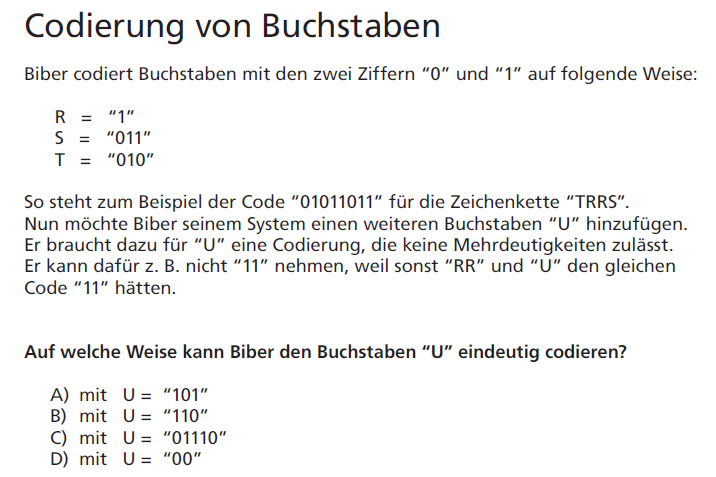
\includegraphics[scale=0.6]{BiberCode.png}
\end{figure}
\pause
D) ist richtig
\end{frame}


\begin{frame}
\textbf{Fano-Bedingung}: Wenn kein Codewort Anfangswort eines anderen Codewortes ist,
dann ist jede codierte Zeichenreihe eindeutig dekodierbar.

Der Huffman-Algorithmus führt zu einer Codierung, die die Fano-Bedingung erfüllt und die
beweisbar die größtmögliche Komprimierung erreicht.
\end{frame}

\begin{frame}
Wir wollen das Wort \textit{regenwetter} mit dem Huffman-Algorithmus codieren.  \pause
Dazu zählen wir, wie oft die verschiedenen Buchstaben in dem Text vorkommen.   
\begin{tikzpicture}
\node (2) at (7,0) [circle, draw] {$2$};
\node (r) at (7,-1) [rectangle, draw] {$r$} 		edge[-] (2);

\node (4) at (9,0) [circle, draw] {$4$};
\node (e) at (9,-1) [rectangle, draw] {$e$}  edge[-] (4);

\node (1) at (11,0) [circle, draw] {$1$};
\node (g) at (11,-1) [rectangle, draw] {$g$}  edge[-] (1);

\node (1a) at (13,0) [circle, draw] {$1$};
\node (n) at (13,-1) [rectangle, draw] {$n$}  edge[-] (1a);

\node (1b) at (15,0) [circle, draw] {$1$};
\node (w) at (15,-1) [rectangle, draw] {$w$} edge[-] (1b);

\node (2a) at (17,0) [circle, draw] {$2$};
\node (t) at (17,-1) [rectangle, draw] {$t$} edge[-] (2a);
\end{tikzpicture}	  

Wir betrachten das Ergebnis als eine Liste von Bäumen.  
Von links gehen wir durch die Liste und suchen die beiden Bäume mit den kleinsten Zahlen in der Wurzel.   
Das sind in unserem Fall die Bäume, an denen das g und das n hängen.  Diese werden linker und rechter Teilbaum eines neuen Baums, in dessen Wurzel wir die Summe der beiden Zahlen schreiben.  Der neue Baum wird rechts an die Liste angefügt. Die beiden benutzen Bäume verschwinden aus der Liste.
\\
\end{frame}
\begin{frame}
\begin{tikzpicture}
\node (2) at (7,0) [circle, draw] {$2$};
\node (r) at (7,-1) [rectangle, draw] {$r$} 		edge[-] (2);

\node (4) at (9,0) [circle, draw] {$4$};
\node (e) at (9,-1) [rectangle, draw] {$e$}  edge[-] (4);

\node (1) at (11,0) [circle, draw] {$1$};
\node (g) at (11,-1) [rectangle, draw] {$g$}  edge[-] (1);

\node (1a) at (13,0) [circle, draw] {$1$};
\node (n) at (13,-1) [rectangle, draw] {$n$}  edge[-] (1a);

\node (1b) at (15,0) [circle, draw] {$1$};
\node (w) at (15,-1) [rectangle, draw] {$w$} edge[-] (1b);

\node (2a) at (17,0) [circle, draw] {$2$};
\node (t) at (17,-1) [rectangle, draw] {$t$} edge[-] (2a);
\end{tikzpicture}	

\begin{tikzpicture}
\node (2) at (7,0) [circle, draw] {$2$};
\node (r) at (7,-1) [rectangle, draw] {$r$} 		edge[-] (2);

\node (4) at (9,0) [circle, draw] {$4$};
\node (e) at (9,-1) [rectangle, draw] {$e$}  edge[-] (4);

\node (1b) at (11,0) [circle, draw] {$1$};
\node (w) at (11,-1) [rectangle, draw] {$w$} edge[-] (1b);

\node (2a) at (13,0) [circle, draw] {$2$};
\node (t) at (13,-1) [rectangle, draw] {$t$} edge[-] (2a);

\node (2b) at (15,0) [circle, draw] {$2$};
      \node (1) at (14.5,-1) [circle, draw] {$1$} edge[-] (2b);
	\node (g) at (14.5,-2) [rectangle, draw] {$g$} 		edge[-] (1);

      \node (1a) at (15.5,-1) [circle, draw] {$1$} edge[-] (2b); 
	\node (n) at (15.5,-2) [rectangle, draw] {$n$} 		edge[-] (1a);
\end{tikzpicture}

Wir wiederholen diesen Schritt, bis nur noch ein Baum übrigbleibt.
\end{frame}

\begin{frame}
\begin{tikzpicture}
\node (2) at (7,0) [circle, draw] {$2$};
\node (r) at (7,-1) [rectangle, draw] {$r$} 		edge[-] (2);

\node (4) at (9,0) [circle, draw] {$4$};
\node (e) at (9,-1) [rectangle, draw] {$e$}  edge[-] (4);

\node (1b) at (11,0) [circle, draw] {$1$};
\node (w) at (11,-1) [rectangle, draw] {$w$} edge[-] (1b);

\node (2a) at (13,0) [circle, draw] {$2$};
\node (t) at (13,-1) [rectangle, draw] {$t$} edge[-] (2a);

\node (2b) at (15,0) [circle, draw] {$2$};
      \node (1) at (14.5,-1) [circle, draw] {$1$} edge[-] (2b);
	\node (g) at (14.5,-2) [rectangle, draw] {$g$} 		edge[-] (1);

      \node (1a) at (15.5,-1) [circle, draw] {$1$} edge[-] (2b); 
	\node (n) at (15.5,-2) [rectangle, draw] {$n$} 		edge[-] (1a);
\end{tikzpicture}

\begin{tikzpicture}
\node (4) at (7,0) [circle, draw] {$4$};
\node (e) at (7,-1) [rectangle, draw] {$e$}  edge[-] (4);

\node (2a) at (9,0) [circle, draw] {$2$};
\node (t) at (9,-1) [rectangle, draw] {$t$} edge[-] (2a);

\node (2b) at (11,0) [circle, draw] {$2$};
      \node (1) at (10.5,-1) [circle, draw] {$1$} edge[-] (2b);
	\node (g) at (10.5,-2) [rectangle, draw] {$g$} 		edge[-] (1);

      \node (1a) at (11.5,-1) [circle, draw] {$1$} edge[-] (2b); 
	\node (n) at (11.5,-2) [rectangle, draw] {$n$} 		edge[-] (1a);

\node (3) at (13,0) [circle, draw] {$3$};
	\node (2) at (12.5,-1)[circle, draw] {$1$} edge[-] (3);
	\node (w) at (12.5,-2) [rectangle, draw] {$w$} 		edge[-] (2);

	\node (1b) at (13.5,-1) [circle, draw] {$2$} edge[-] (3);
	\node (r) at (13.5,-2) [rectangle, draw] {$r$} edge[-] (1b);
\end{tikzpicture}	
\end{frame}

\begin{frame}

\begin{tikzpicture}
\node (4) at (7,0) [circle, draw] {$4$};
\node (e) at (7,-1) [rectangle, draw] {$e$}  edge[-] (4);

\node (2a) at (9,0) [circle, draw] {$2$};
\node (t) at (9,-1) [rectangle, draw] {$t$} edge[-] (2a);

\node (2b) at (11,0) [circle, draw] {$2$};
      \node (1) at (10.5,-1) [circle, draw] {$1$} edge[-] (2b);
	\node (g) at (10.5,-2) [rectangle, draw] {$g$} 		edge[-] (1);

      \node (1a) at (11.5,-1) [circle, draw] {$1$} edge[-] (2b); 
	\node (n) at (11.5,-2) [rectangle, draw] {$n$} 		edge[-] (1a);

\node (3) at (13,0) [circle, draw] {$3$};
	\node (2) at (12.5,-1)[circle, draw] {$1$} edge[-] (3);
	\node (w) at (12.5,-2) [rectangle, draw] {$w$} 		edge[-] (2);

	\node (1b) at (13.5,-1) [circle, draw] {$2$} edge[-] (3);
	\node (r) at (13.5,-2) [rectangle, draw] {$r$} edge[-] (1b);
\end{tikzpicture}	

\begin{tikzpicture}
\node (4) at (7,0) [circle, draw] {$4$};
\node (e) at (7,-1) [rectangle, draw] {$e$}  edge[-] (4);

\node (3) at (9,0) [circle, draw] {$3$};
	\node (2) at (8.5,-1)[circle, draw] {$1$} edge[-] (3);
	\node (w) at (8.5,-2) [rectangle, draw] {$w$} 		edge[-] (2);

	\node (1b) at (9.5,-1) [circle, draw] {$2$} edge[-] (3);
	\node (r) at (9.5,-2) [rectangle, draw] {$r$} edge[-] (1b);

\node (4a) at (11.25,0) [circle, draw] {$4$};	
	\node (2a) at (10.5,-1) [circle, draw] {$2$}  edge[-] (4a);			
	\node (t) at (10.5,-2) [rectangle, draw] {$t$} edge[-] (2a);

	\node (2b) at (12,-1) [circle, draw] {$2$}  edge[-] (4a);		;
     		 \node (1) at (11.5,-2) [circle, draw] {$1$} edge[-] (2b);
	       \node (g) at (11.5,-3) [rectangle, draw] {$g$} 		edge[-] (1);
	
    		 \node (1a) at (12.5,-2) [circle, draw] {$1$} edge[-] (2b); 
		 \node (n) at (12.5,-3) [rectangle, draw] {$n$} 		edge[-] (1a);

\end{tikzpicture}	
\end{frame}

\begin{frame}
\begin{tikzpicture}
\node (4) at (7,0) [circle, draw] {$4$};
\node (e) at (7,-1) [rectangle, draw] {$e$}  edge[-] (4);

\node (3) at (9,0) [circle, draw] {$3$};
	\node (2) at (8.5,-1)[circle, draw] {$1$} edge[-] (3);
	\node (w) at (8.5,-2) [rectangle, draw] {$w$} 		edge[-] (2);

	\node (1b) at (9.5,-1) [circle, draw] {$2$} edge[-] (3);
	\node (r) at (9.5,-2) [rectangle, draw] {$r$} edge[-] (1b);

\node (4a) at (11.25,0) [circle, draw] {$4$};	
	\node (2a) at (10.5,-1) [circle, draw] {$2$}  edge[-] (4a);			
	\node (t) at (10.5,-2) [rectangle, draw] {$t$} edge[-] (2a);

	\node (2b) at (12,-1) [circle, draw] {$2$}  edge[-] (4a);		;
     		 \node (1) at (11.5,-2) [circle, draw] {$1$} edge[-] (2b);
	       \node (g) at (11.5,-3) [rectangle, draw] {$g$} 		edge[-] (1);
	
    		 \node (1a) at (12.5,-2) [circle, draw] {$1$} edge[-] (2b); 
		 \node (n) at (12.5,-3) [rectangle, draw] {$n$} 		edge[-] (1a);

\end{tikzpicture}	

\begin{tikzpicture}
\node (4a) at (11.25-3,0) [circle, draw] {$4$};	
	\node (2a) at (10.5-3,-1) [circle, draw] {$2$}  edge[-] (4a);			
	\node (t) at (10.5-3,-2) [rectangle, draw] {$t$} edge[-] (2a);

	\node (2b) at (12-3,-1) [circle, draw] {$2$}  edge[-] (4a);		;
     		 \node (1) at (11.5-3,-2) [circle, draw] {$1$} edge[-] (2b);
	       \node (g) at (11.5-3,-3) [rectangle, draw] {$g$} 		edge[-] (1);
	
    		 \node (1a) at (12.5-3,-2) [circle, draw] {$1$} edge[-] (2b); 
		 \node (n) at (12.5-3,-3) [rectangle, draw] {$n$} 		edge[-] (1a);

\node (7) at (12.5,0) [circle, draw] {$7$};	
	\node (4) at (10+3.75,-1) [circle, draw] {$4$} edge[-] (7);
	\node (e) at (10+3.75,-2) [rectangle, draw] {$e$}  edge[-] (4);


	\node (3) at (8+3.5,-1) [circle, draw] {$3$}  edge[-] (7);
		\node (2) at (7.5+3.5,-2)[circle, draw] {$1$} edge[-] (3);
		\node (w) at (7.5+3.5,-3) [rectangle, draw] {$w$} 		edge[-] (2);

		\node (1b) at (8.5+3.5,-2) [circle, draw] {$2$} edge[-] (3);
		\node (r) at (8.5+3.5,-3) [rectangle, draw] {$r$} edge[-] (1b);
\end{tikzpicture}	
\end{frame}

\begin{frame}

\begin{tikzpicture}
\node (4a) at (11.25-3,0) [circle, draw] {$4$};	
	\node (2a) at (10.5-3,-1) [circle, draw] {$2$}  edge[-] (4a);			
	\node (t) at (10.5-3,-2) [rectangle, draw] {$t$} edge[-] (2a);

	\node (2b) at (12-3,-1) [circle, draw] {$2$}  edge[-] (4a);		;
     		 \node (1) at (11.5-3,-2) [circle, draw] {$1$} edge[-] (2b);
	       \node (g) at (11.5-3,-3) [rectangle, draw] {$g$} 		edge[-] (1);
	
    		 \node (1a) at (12.5-3,-2) [circle, draw] {$1$} edge[-] (2b); 
		 \node (n) at (12.5-3,-3) [rectangle, draw] {$n$} 		edge[-] (1a);

\node (7) at (12.5,0) [circle, draw] {$7$};	
	\node (4) at (10+3.75,-1) [circle, draw] {$4$} edge[-] (7);
	\node (e) at (10+3.75,-2) [rectangle, draw] {$e$}  edge[-] (4);


	\node (3) at (8+3.5,-1) [circle, draw] {$3$}  edge[-] (7);
		\node (2) at (7.5+3.5,-2)[circle, draw] {$1$} edge[-] (3);
		\node (w) at (7.5+3.5,-3) [rectangle, draw] {$w$} 		edge[-] (2);

		\node (1b) at (8.5+3.5,-2) [circle, draw] {$2$} edge[-] (3);
		\node (r) at (8.5+3.5,-3) [rectangle, draw] {$r$} edge[-] (1b);
\end{tikzpicture}	
\begin{tikzpicture}
\node (11) at (10.5,0) [circle, draw] {$11$};

\node (4a) at (11.25-3,-1) [circle, draw] {$4$}  edge[-] (11);
	\node (2a) at (10.5-3,-2) [circle, draw] {$2$}  edge[-] (4a);			
	\node (t) at (10.5-3,-3) [rectangle, draw] {$t$} edge[-] (2a);

	\node (2b) at (12-3,-2) [circle, draw] {$2$}  edge[-] (4a);		;
     		 \node (1) at (11.5-3,-3) [circle, draw] {$1$} edge[-] (2b);
	       \node (g) at (11.5-3,-4) [rectangle, draw] {$g$} 		edge[-] (1);
	
    		 \node (1a) at (12.5-3,-3) [circle, draw] {$1$} edge[-] (2b); 
		 \node (n) at (12.5-3,-4) [rectangle, draw] {$n$} 		edge[-] (1a);

\node (7) at (12.5,-1) [circle, draw] {$7$}  edge[-] (11);	
	\node (4) at (10+3.75,-2) [circle, draw] {$4$} edge[-] (7);
      \node (e) at (10+3.75,-3) [rectangle, draw] {$e$}  edge[-] (4);


	\node (3) at (8+3.5,-2) [circle, draw] {$3$}  edge[-] (7);
	    	\node (2) at (7.5+3.5,-3)[circle, draw] {$1$} edge[-] (3);
		\node (w) at (7.5+3.5,-4) [rectangle, draw] {$w$} 		edge[-] (2);

		\node (1b) at (8.5+3.5,-3) [circle, draw] {$2$} edge[-] (3);
		\node (r) at (8.5+3.5,-4) [rectangle, draw] {$r$} edge[-] (1b);

\end{tikzpicture}
\end{frame}
\begin{frame}[fragile]
Wenn nur noch ein Baum vorhanden ist, können wir die Bitmuster für die Codierung der Zeichen ablesen. Abstieg in den linken Teilbaum ergibt 0, Abstieg in den rechten Teilbaum ergibt 1. 

\begin{tikzpicture}
\node (11) at (10.5,0) [circle, draw] {$11$};

\node (4a) at (11.25-3,-1) [circle, draw] {$4$}  edge[-] (11);
	\node (2a) at (10.5-3,-2) [circle, draw] {$2$}  edge[-] (4a);			
	\node (t) at (10.5-3,-3) [rectangle, draw] {$t$} edge[-] (2a);

	\node (2b) at (12-3,-2) [circle, draw] {$2$}  edge[-] (4a);		;
     		 \node (1) at (11.5-3,-3) [circle, draw] {$1$} edge[-] (2b);
	       \node (g) at (11.5-3,-4) [rectangle, draw] {$g$} 		edge[-] (1);
	
    		 \node (1a) at (12.5-3,-3) [circle, draw] {$1$} edge[-] (2b); 
		 \node (n) at (12.5-3,-4) [rectangle, draw] {$n$} 		edge[-] (1a);

\node (7) at (12.5,-1) [circle, draw] {$7$}  edge[-] (11);	
	\node (4) at (10+3.75,-2) [circle, draw] {$4$} edge[-] (7);
      \node (e) at (10+3.75,-3) [rectangle, draw] {$e$}  edge[-] (4);


	\node (3) at (8+3.5,-2) [circle, draw] {$3$}  edge[-] (7);
	    	\node (2) at (7.5+3.5,-3)[circle, draw] {$1$} edge[-] (3);
		\node (w) at (7.5+3.5,-4) [rectangle, draw] {$w$} 		edge[-] (2);

		\node (1b) at (8.5+3.5,-3) [circle, draw] {$2$} edge[-] (3);
		\node (r) at (8.5+3.5,-4) [rectangle, draw] {$r$} edge[-] (1b);

\end{tikzpicture} 

Wir erhalten folgende Codierung:
\begin{lstlisting}
t = 00, g = 010, n = 011, w = 100, r = 101, e = 11
\end{lstlisting}
\end{frame}


\begin{frame}[fragile]
\begin{lstlisting}
t = 00, g = 010, n = 011, w = 100, r = 101, e = 11
\end{lstlisting} 
Die Codierung von \textit{regenwetter} hat eine Länge von 27 bit:
\begin{lstlisting}
101110101101110011000011101
\end{lstlisting}  
Bei der ASCII-Codierung wird jedes Zeichen mit 8 bit codiert. Für die 11 Buchstaben von  \textit{regenwetter} wären also 88 bit erforderlich. In der Huffman Codierung werden  61 bit, das sind ca. 69\% der ursprünglichen Codierung eingespart.  

Zur Dekodierung muss natürlich der verwendete Huffman-Baum zur Verfügung stehen.
\end{frame}

\end{document}




















